\input ../SlidePreamble
\input ../preamble


\begin{document}

{\Huge
  \centerline{\bf TTIC 31230,  Fundamentals of Deep Learning}
  \vfill
  \centerline{David McAllester, Autumn   2023}
  \vfill
  \centerline{\bf Vector Quantization for Autoregressive Modeling}
  \vfill
  \vfill

\slide{Autoregressive Image and Voice Modeling}

Strong VAE image modeling was first achieved with autoregressive token modeling.

\vfill
\centerline{van den Oord, Vinyals and Kavukcuoglu,}
\centerline{Neural Discrete Representation Learning, {\bf 2017}}

\vfill
\centerline{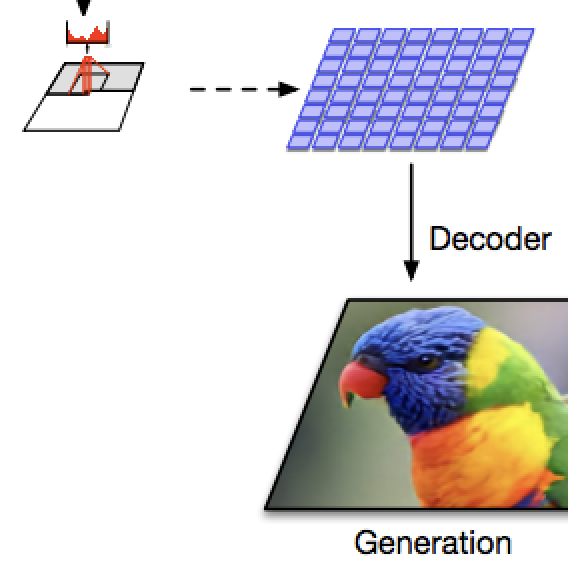
\includegraphics[height = 2in]{\images/VQ-OneLayer} 
\parbox[b]{4.5in}{\huge Token Transformer \\ \\ Image-to-Tokens, Tokens-to-Image \\ \\ \\~}}

\slide{VQ-VAE-2, June 2019}

\centerline{Generating Diverse High-Fidelity Images
with VQ-VAE-2}

\vfill
\centerline{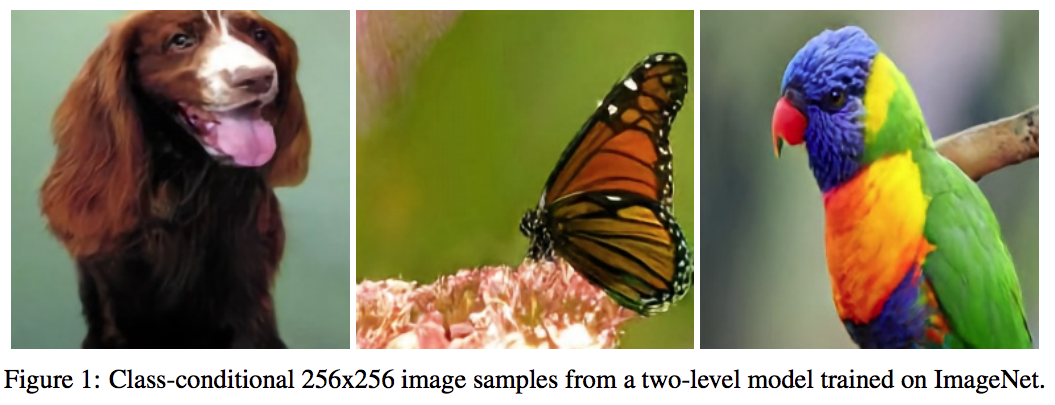
\includegraphics[width = 8in]{\images/VQ-VAE21}}

\slide{VAE Tokenization of Images and Voice}

\centerline{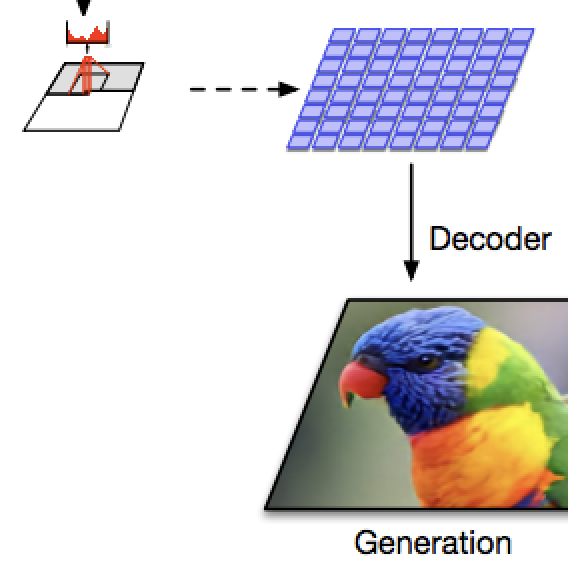
\includegraphics[height = 2in]{\images/VQ-OneLayer} 
\parbox[b]{4.5in}{\huge Token Transformer \\ \\ Image-to-Tokens, Tokens-to-Image \\ \\ \\~}}


\vfill
Let $y$ range over a population (such as images or sound waves).

\vfill
Assume that a given $y$ is encoded as a tensor denoted {\color{red} $z_{\enc,p}(y)$} where $p$ is a ``position in $y$'' (a pixel in an image tensor
or time window in a sound tensor) and {\color{red} $z_{\enc, p}(y) \in R^d$} is a vector.

\slide{Vector Quantization (Tokenization)}

\centerline{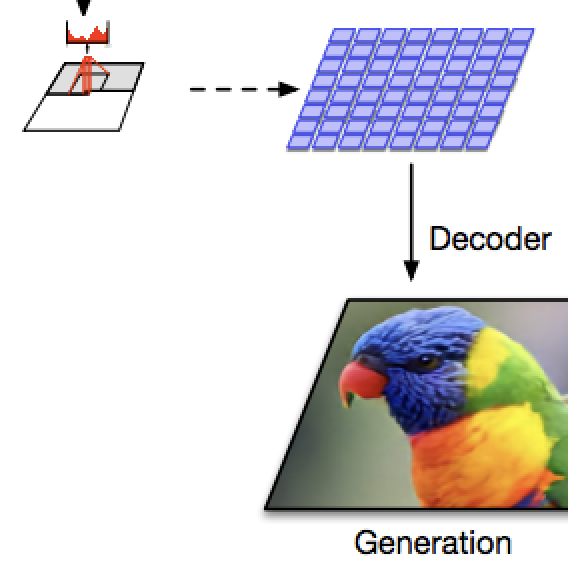
\includegraphics[height = 2in]{\images/VQ-OneLayer} 
\parbox[b]{4.5in}{\huge Token Transformer \\ \\ Image-to-Tokens, Tokens-to-Image \\ \\ \\~}}

\vfill
Assume a finite set of $K$ ``tokens'' where token $k$ has an embedding vector $e(k) \in R^d$.

\vfill
Define $k_{\enc,p}(y)$ by
$$k_{\enc,p}(y)= \argmin_k\;\frac{1}{2}||z_{\enc,p}(y)-e(k)||^2$$

\slide{Reconstruction Loss}

\centerline{\parbox[b]{1.0in}{\huge $P_\pri(k)$ \\ \\ \\ \\ \\ ~}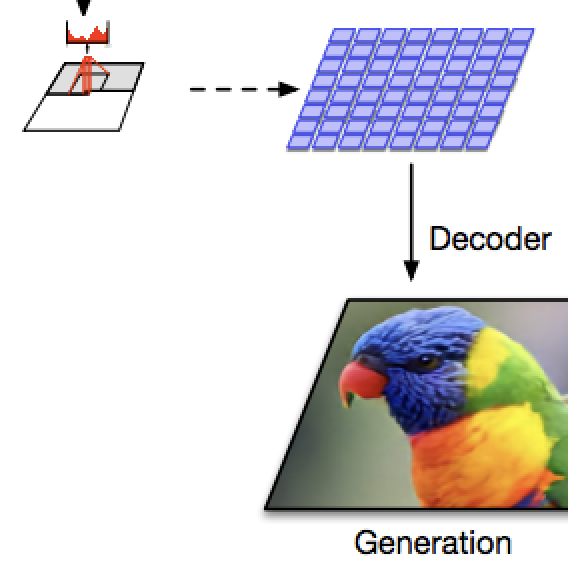
\includegraphics[height = 2in]{\images/VQ-OneLayer} 
\parbox[b]{2.5in}{\huge $k_\enc(y)$ \\ \\ \\ \\ $y$ \\~}}

We now have a VAE where the tensor $k_\enc(y)$ is the latent variable.

\vfill
The encoder and decoder are trained jointly.

\vfill
The prior is a transformer trained after the encoder and decoder are fully trained.

\slide{Training the Encoder and Decoder}
\centerline{\parbox[b]{1.0in}{\huge $P_\pri(k)$ \\ \\ \\ \\ \\ ~}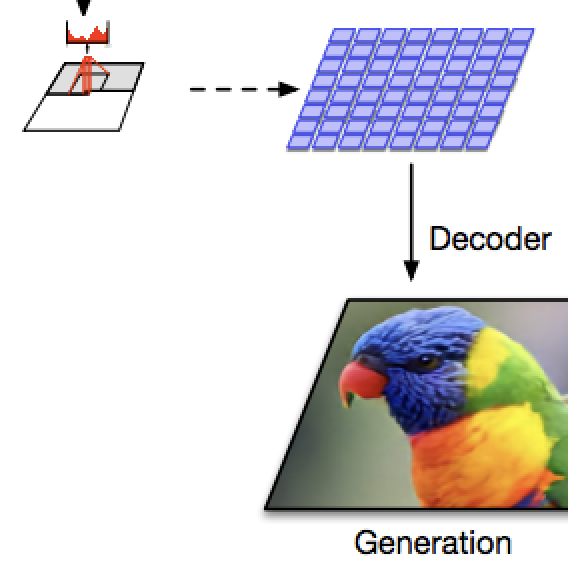
\includegraphics[height = 2in]{\images/VQ-OneLayer} 
\parbox[b]{2.5in}{\huge $k(z_\enc(y))$ \\ \\ \\ \\ $y$ \\~}}

\vfill
Taking $P_\dec(y|k)$ to be ${\cal N}(\hat{y}_\dec(k),I)$ we get an $L_2$ reconstruction loss.

\vfill
$${\cal L}_{\mathrm{Rec}} = \frac{1}{2}||\;y - \hat{y}_\dec(e(k(z_\enc(y))))\;||^2$$

\slide{Training the Encoder and Decoder}
\centerline{\parbox[b]{1.0in}{\huge $P_\pri(k)$ \\ \\ \\ \\ \\ ~}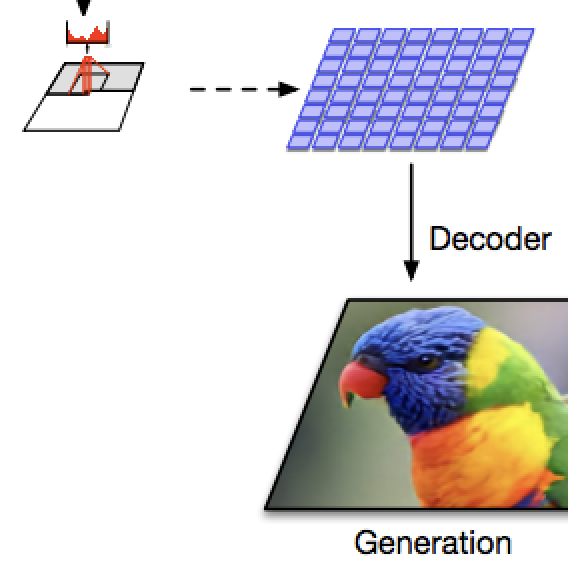
\includegraphics[height = 2in]{\images/VQ-OneLayer} 
\parbox[b]{2.5in}{\huge $k(z_\enc(y))$ \\ \\ \\ \\ $y$ \\~}}

\vfill
$${\cal L}_{\mathrm{Rec}} = \frac{1}{2}||\;y - \hat{y}_\dec(e(k(z_\enc(y))))\;||^2$$

\vfill
Because the tokens are discrete we do not get any gradient on $z_\enc(y)$.

\slide{Straight-Through Gradients}
\centerline{\parbox[b]{1.0in}{\huge $P_\pri(k)$ \\ \\ \\ \\ \\ ~}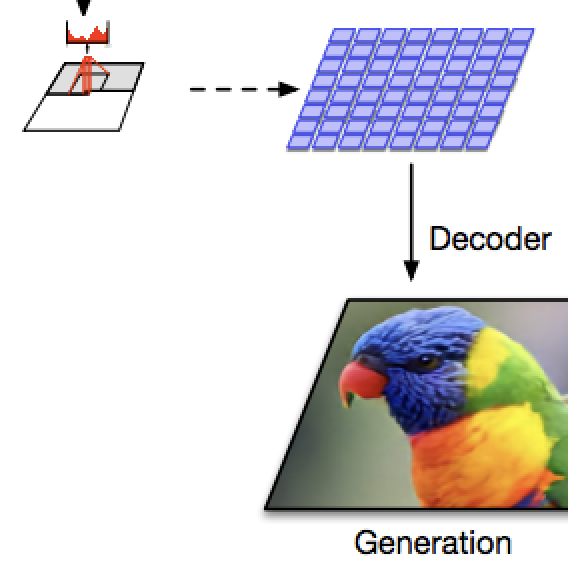
\includegraphics[height = 2in]{\images/VQ-OneLayer} 
\parbox[b]{2.5in}{\huge $k(z_\enc(y))$ \\ \\ \\ \\ $y$ \\~}}

\vfill
$${\cal L}_{\mathrm{Rec}} = \frac{1}{2}||\;y - \hat{y}_\dec(e(k(z_\enc(y))))\;||^2$$

\vfill{
$$z_{\enc,p}(y).\grad = \nabla_{e(k(z_{\enc,p}(y)))} {\cal L}_{\mathrm{Rec}}$$

\slide{K-Means Gradients}

We train $z_\enc(y)$ and the token embeddings $e(k)$.

\vfill
$${\cal L}_{\mathrm{Rec}} = \frac{1}{2}||\;y - \hat{y}_\dec(e(k(z_\enc(y))))\;||^2$$

\vfill{
$$z_{\enc,p}(y).\grad = \nabla_{e(k(z_{\enc,p}(y)))} {\cal L}_{\mathrm{Rec}}$$

\vfill
$${\cal L}_{\mathrm{KM}} = \frac{1}{2}||z_{\enc,p}(y) - e(k(z_{\enc,p}))||^2$$

\vfill{
$$e(k(z_{\enc,p}(y))).\grad \;\pluseq\; \beta \nabla_{e(k(z_{\enc,p}(y)))} {\cal L}_{\mathrm{KM}}$$

\vfill
$\beta$ is a hyper-parameter that adjust the relative learning rates.

\slide{Transformer Training}

Finally we hold the encoder fixed and train the prior $P_\pri(z)$ to be an auto-regressive model of the symbolic image $k_\enc(s)[X,Y]$.

\vfill
\centerline{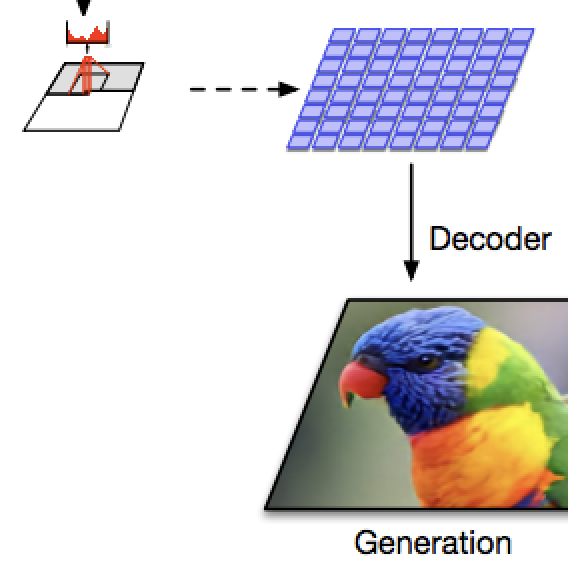
\includegraphics[height = 2in]{\images/VQ-OneLayer}}

\slide{Tokenization and Gaussian Mixture Models (GMMs)}

Consider modeling $P(y|x)$ with $y \in R^d$

\vfill
A Gaussian model has the form

\begin{eqnarray*}
y & = & \hat{y}(x) + \sigma \epsilon,\;\;\;\epsilon \sim {\cal N}(0,I) \\
\\
\hat{y} & = & \argmin_{\hat{y}}\; E_{x,y}\;||\hat{y}(x)-y||^2
\end{eqnarray*}

\slide{Tokenization and Gaussian Mixture Models (GMMs)}

Now consider a tokenizing decoder

\begin{eqnarray*}
y & = & E_{k\sim P_\dec(k|x)}[\; e(k) + \sigma \epsilon\;],\;\;\;\epsilon \sim {\cal N}(0,I) \\
\end{eqnarray*}

We get that $P_\dec(y|x)$ is a Gaussian mixture model (GMM).

\vfill
GMMs are significantly more expressive than single Gaussians.

\vfill

\slide{Wav2Vec 2.0, June 2020, Facebook}

\vfill
Trained on 53k hours of unlabeled audio (no text) they convert speech to a sequence of discrete quantized vectors they call ``pseudo-text units''.

\vfill
By training on only one hour of human-transcribed audio, and using the Wav2Vec transcription into pseudo-text, they outperform the previous state of the
art in word error rate for 100 hours of human-transcribed text.

\slide{DALLE-1, January 2021}

\vfill
\centerline{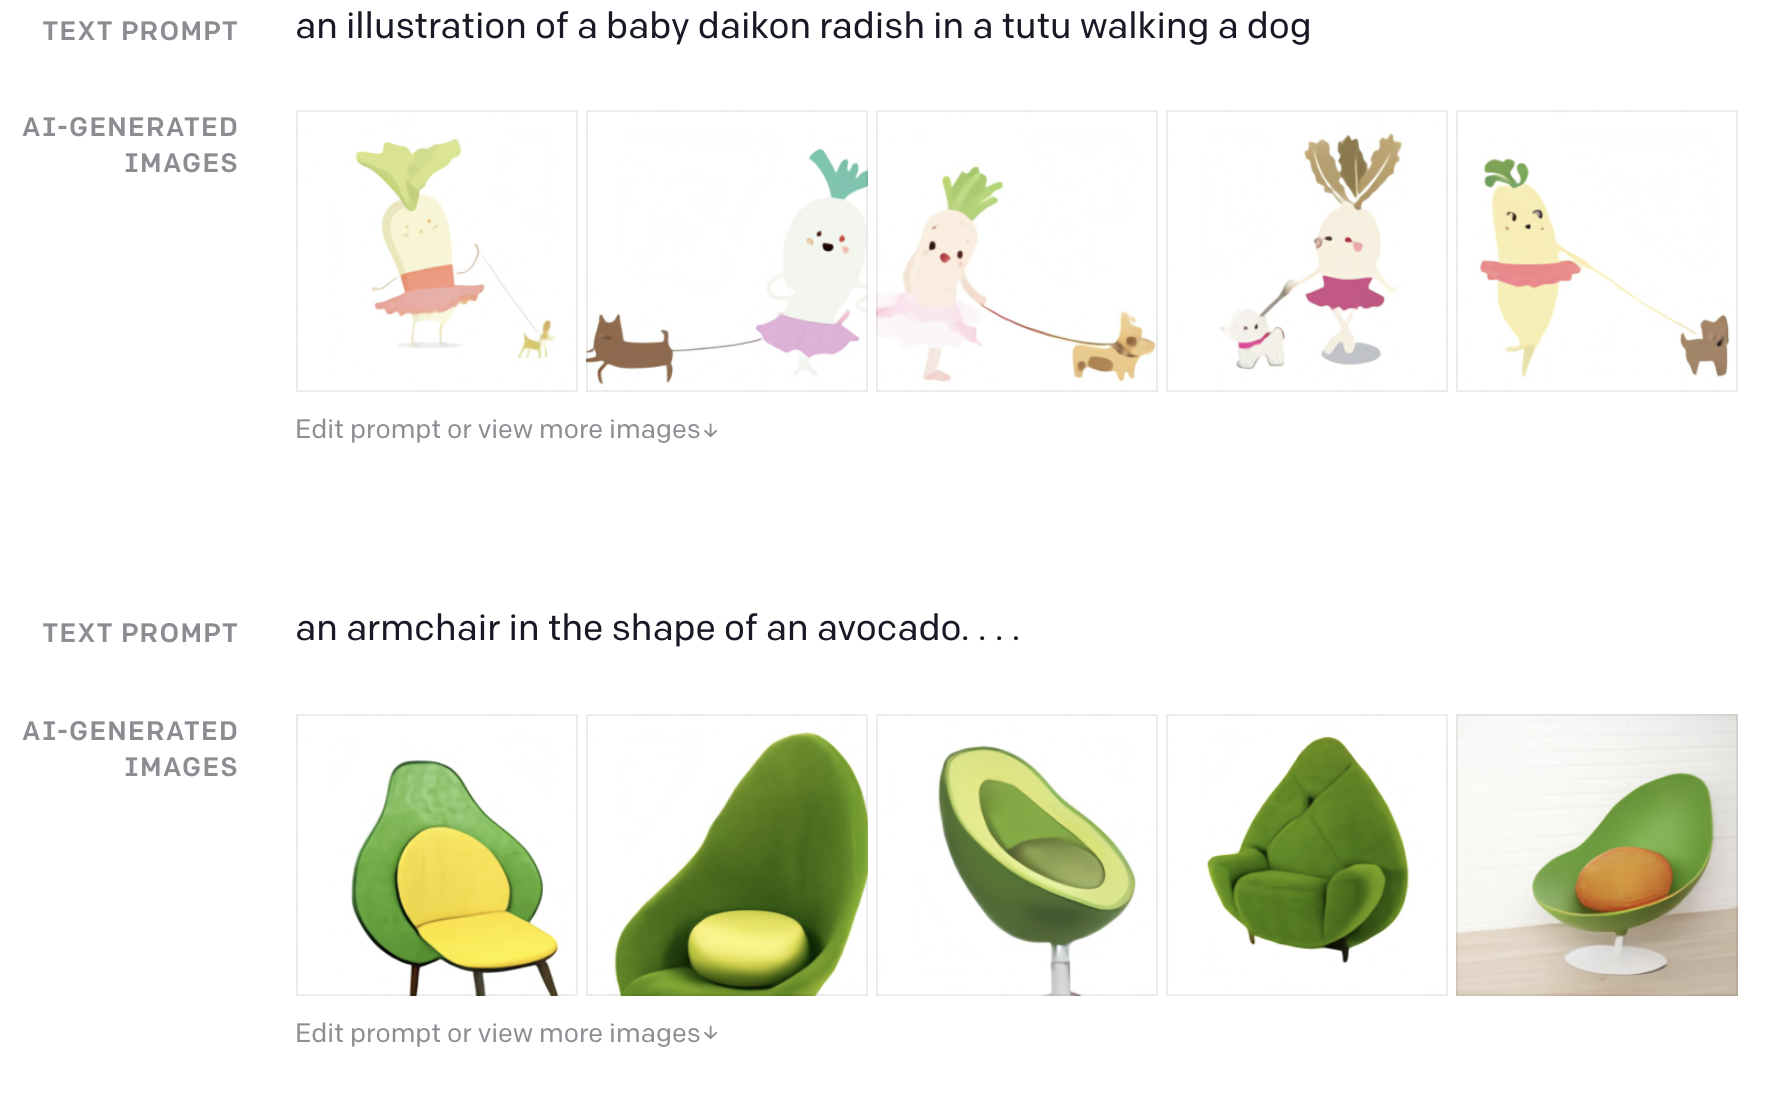
\includegraphics[width = 8in]{\images/DALLE1}}


\slide{GLSM, February 2021, Facebook}

Generative Spoken Language Model (GSLM)

\vfill
They then train a generative model of the sequences of pseudo-text units learned from unlabeled audio.


\vfill
This model can continue speech from a speech prompt in much the same way that GPT-3 continues text from a text prompt.

\vfill
Semantic and grammatical structure in a ``unit language model'' is recovered
from speech alone.

\slide{Parti, June 2022}

\centerline{\huge Scaling Autoregressive Models for Content-Rich Text-to-Image Generation}
\centerline{\huge Yu et al.}

\vfill
\centerline{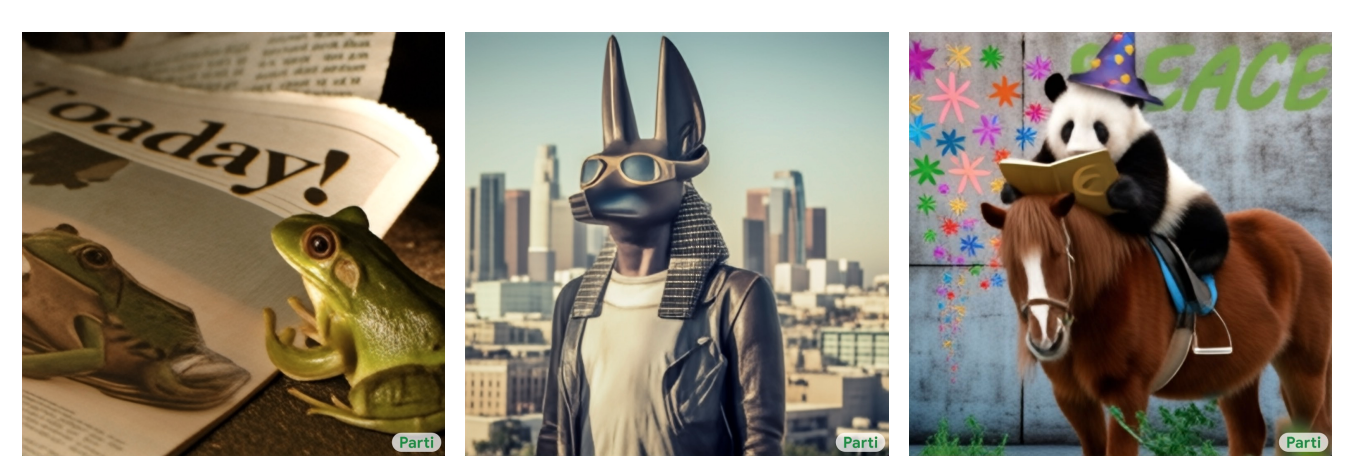
\includegraphics[width = 9in]{\images/Parti}}


\slide{CM3Leon, September 2023}

\centerline{\Large Scaling Autoregressive Multi-Modal Models: Pretraining and Instruction Tuning}
\centerline{\Large Yu et al.}

\vfill
\centerline{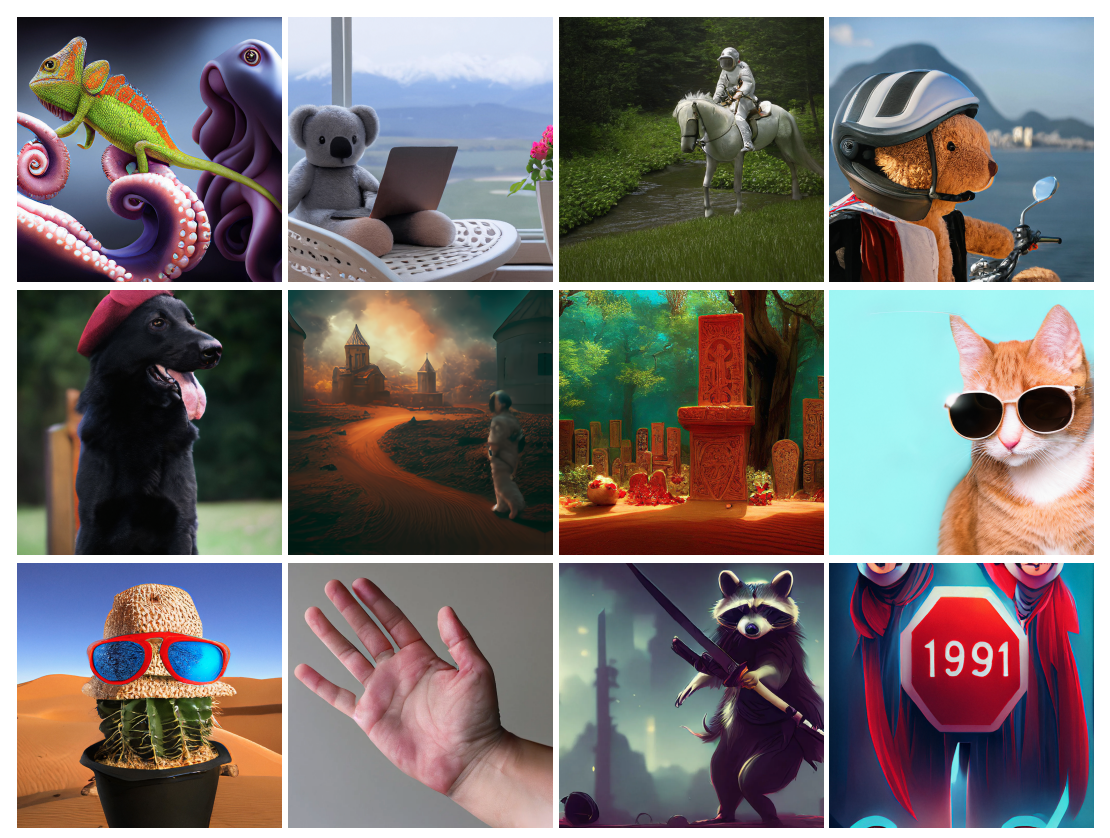
\includegraphics[width = 5.7in]{\images/CM3Leon}}


\slide{Voice-Text Language Model (VoxtLM), September 2023}

This is similar to CM3Leon but for voice and text rather than images and text.

\vfill
Voice is tokenized and then a transformer is used to model sequences that alternate voice and text.



\slide{END}

}
\end{document}

